\chapter{Auswertung}
\label{cha:Auswertung}
Die in diesem Kapitel genannten Standardfehler des Mittelwertes ergeben sich nach
\begin{equation*}
  \label{eqn:MW-Fehler}
  \sigma(x) = \sqrt{\frac{1}{n(n-1)} \sum_i (x_i - \overline{x})^2}.
\end{equation*}
Daraus resultierende Unsicherheiten genügen der Gaußschen Fehlerfortpflanzung.
Die Fehlerrechnung wird in \textit{Python} unter Verwendung des Paketes \textit{uncertainties} \cite{uncertainties} durchgeführt.

\section{Kontrastmessung}
\label{sec:kontrastmessung}
Nun wird der Kontrast in Abhängigkeit des Polarisationswinkels bestimmt. Wie bereits in \autoref{sec:Kontrast} diskutiert wird der Kontrast durch Gleichung \ref{eqn:kontrast} berechnet.
Im selben Abschnitt wurde dann auch die Proportionalität der Intensität zum Winkel erklärt. Führt man diese Proportionalität in Gleichung \ref{eqn:kontrast} ein erhält man eine 
theoretische Winkelabhänigkeit des Kontrastes, dessen Form in durch Gleichung \ref{eqn:kontrast_phi} gegeben ist. Die Messwerte sind in Abbildung \ref{fig:kontrast} dargestellt. Mittels
einer Regression durch \textit{Scipy}\cite{scipy} wurde der Parameter a zu $a = \num{1.9796}$ bestimmt. 

\begin{equation}
  \label{eqn:kontrast_phi}
  K = a\lvert \cos(\Phi)\sin(\Phi)\rvert  
\end{equation}
\begin{figure}
    \centering
    \includegraphics{kontrast.pdf}
    \caption{In dieser Abbildung wird die Winkelabhänigkeit des Kontrastes eines Sagnac-Interferometers dargestellt.}
    \label{fig:kontrast}
\end{figure}

Aus den Messdaten in Abbildung \ref{fig:kontrast} lässt sich einer maximaler Kontrast $K_\mathrm{max} = 0.9608$ entnehmen, welcher bei einem Winkel $\Phi = \qty{50}{\degree}$ auftritt.
Außerdem treten weitere Maxima des Kontrastes bei vielfachen des Winkels auf. Dieses Verhalten ist in anbetracht des periodischen Verhaltens dieses Phänomens logisch. 
Für die folgenden Messungen wurde der Kontrast nun auf das Maxima eingestellt, wie bereits in \autoref{cha:Durchführung} erwähnt. Im folgenden wird die Differenzspannungsmethode 
verwendet.

\section{Brechungsindex von Glas}
\label{sec:n_glas}
Der Brechungsindex von Glas wird durch zwei Glasplättchen, welche jeweils in einem der Strahlengänge liegen gemessen. Der Brechungsindex lässt sich nach Modifikation von Gleichung 
\ref{eq:Phi} durch Gleichung \ref{eq:Maxima} beschrieben. In dieser Gleichung ist $T = \qty{1}{\milli\metre}$ die Dicke eine Glasplatte, $M$ die Anzahl der Interferenzmaxima oder 
Minima, $\lambda_\mathrm{vac} = \qty{632.990}{\nano\metre}$ die Wellenlänge des Lichtes im Vakuum, $\Theta_0 = \qty{\pm 10}{\degree}$ die Drehung der Spiegel und 
$\Theta = \qty{10}{\degree}$ ist der Drehwinkel des Doppelglashalters. Damit lässt sich der Brechungsindex berechnen. Die aufgenommenen Daten werden in Tabelle \ref{tab:n_glas} 
dargestellt.

\begin{table}[htbp] 
  \centering 
  \begin{tabular}{c c} 
      \toprule $M$ & $n_\mathrm{Glas}$\\ 
      \midrule 
      31 & 1.4751 \\
      31 & 1.4751 \\
      36 & 1.5975 \\
      34 & 1.5462 \\
      34 & 1.5462 \\
      32 & 1.4981 \\
      33 & 1.5218 \\
      32 & 1.4981 \\
      32 & 1.4981 \\
      35 & 1.5715 \\

      \bottomrule 
  \end{tabular} 
  \caption[Tabelle]{In dieser Tabelle sind die experimentell bestimmten Brechungsindex der Glasplättchen aufgetragen.} 
  \label{tab:n_glas} 
\end{table}

Der mittlere Brechungsindex ergibt sich zu $\overline{n}_\mathrm{Glas} = \num{1.5228 \pm 0.0124}$. Der Theoriewert von normalen Fensterglas lautet $\num{1.52}$\cite{phy-chem-eigenschaften}.

\section{Brechungsindex von Luft}
\label{sec:n_luft}
Zuletzt wird der Brechungsindex von Luft bestimmt. Dazu wurde eine Gaszelle mit der Länge $L = \qty{100 \pm 0.1}{\milli\metre}$ verwendet. Die Messungen wurden bei einer Umgebungstemperatur 
von $T = \qty{22}{\celsius}$ aufgenommen. Die Druckmessung wurde bei einem Druck von 
$p_0 = \qty{10}{\milli\bar}$ begonnen und dann wurden bis zu einem Umgebungsdruck $p = \qty{960}{\milli\bar}$ die Intensitätsmaxima $M$ gemessen. Der Brechungsindex von Luft wird gemäß 
Gleichung \ref{eqn:luft} berechnet. Die gemessenen Werte sind in Tabelle \ref{tab:n_luft} dargestellt.

\begin{table}[htbp] 
  \centering 
  \begin{tabular}{c c c c c c c} 
      \toprule $p$ & $M_1$ & $M_2$ & $M_3$ & $n_{\mathrm{Luft},1}$ & $n_{\mathrm{Luft},2}$ & $n_{\mathrm{Luft},3}$ \\ 
      \midrule 
       10 &  0 &  0 &  0 & 1.00000000 & 1.00000000 & 1.00000000 \\
       60 &  2 &  2 &  2 & 1.00001266 & 1.00001266 & 1.00001266 \\
      110 &  4 &  4 &  4 & 1.00002532 & 1.00002532 & 1.00002532 \\
      160 &  6 &  6 &  6 & 1.00003798 & 1.00003798 & 1.00003798 \\
      210 &  8 &  8 &  8 & 1.00005064 & 1.00005064 & 1.00005064 \\
      260 & 10 & 10 & 10 & 1.00006330 & 1.00006330 & 1.00006330 \\
      310 & 12 & 12 & 12 & 1.00007596 & 1.00007596 & 1.00007596 \\
      360 & 14 & 15 & 14 & 1.00008862 & 1.00009495 & 1.00008862 \\
      410 & 17 & 17 & 17 & 1.00010761 & 1.00010761 & 1.00010761 \\
      460 & 19 & 19 & 19 & 1.00012027 & 1.00012027 & 1.00012027 \\
      510 & 21 & 21 & 21 & 1.00013293 & 1.00013293 & 1.00013293 \\
      560 & 23 & 23 & 23 & 1.00014559 & 1.00014559 & 1.00014559 \\
      610 & 25 & 25 & 25 & 1.00015825 & 1.00015825 & 1.00015825 \\
      660 & 28 & 27 & 27 & 1.00017724 & 1.00017091 & 1.00017091 \\
      710 & 30 & 29 & 30 & 1.00018990 & 1.00018357 & 1.00018990 \\
      760 & 32 & 31 & 32 & 1.00020256 & 1.00019623 & 1.00020256 \\
      810 & 34 & 34 & 34 & 1.00021522 & 1.00021522 & 1.00021522 \\
      860 & 37 & 36 & 36 & 1.00023421 & 1.00022788 & 1.00022788 \\
      910 & 39 & 38 & 38 & 1.00024687 & 1.00024054 & 1.00024054 \\
      960 & 41 & 40 & 40 & 1.00025953 & 1.00025320 & 1.00025320 \\
      \bottomrule 
  \end{tabular} 
  \caption[Tabelle]{In dieser Tabelle ist der experimentell bestimmte Brechungsindex von Luft dargestellt. Dabei bezieht sich der Zählindex auf die Nummer der Durchgeführten Messung.} 
  \label{tab:n_luft} 
\end{table}

Daraus ergibt sich ein mittlerer Brechungsindex von Luft zu $n_\mathrm{Luft} = \num{1.00013 \pm 0.00005}$.Dieser Wert gilt allerdings lediglich bei angegeben Raumtemperatur und normalem Druck. Der Theoriewert zum Brechungsindex von Luft ist durch $n_{\mathrm{L,Theo}} = 1.000292$ \cite{Ingenieurwissen}
gegeben. Der experimentell bestimmte Wert wurde allerdings für die angegebene Raumtemperatur bestimmt. Der Theoriewert hingegen für \textit{Normatmosphäre}. Um aus dem bestimmten 
Wert den Brechungsindex von Luft bei Normatmosphäre zu bestimmen kann nun die theoretische Gleichung \ref{eqn:lorentz} genutzt werden. An diese  errechneten 
Daten des Brechungsindex wird die Gleichung gefittet. Die Parameter $\overline{a} = \frac{3}{2}A = \num{0.0006659 \pm 0.0000022}$ und $b = \num{0.9999947 \pm 0.0000005}$ wurden bestimmt. Dabei is $b$
der Achsenabschnitt, welcher nach Theorie gleich $1$ seien sollte. Der Fit mit diesen Parametern wird in \autoref{fig:lorentz} dargestellt.

\begin{figure}
  \centering
  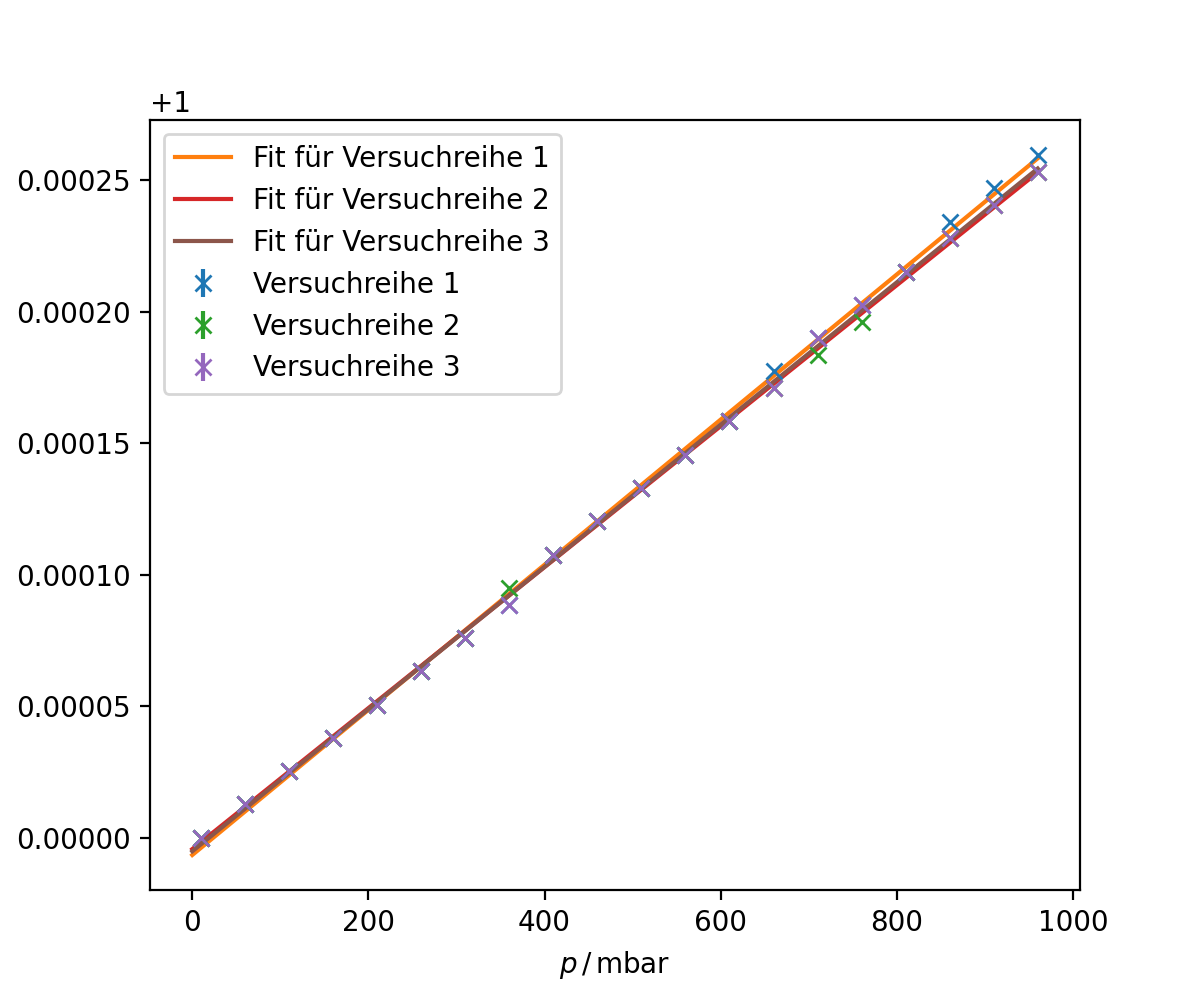
\includegraphics{Fits.pdf}
  \caption{In dieser Abbildung wird der Brechungsindex in Abhängigkeit des Druckes dargestellt.}
  \label{fig:lorentz}
\end{figure}

Mit diesen Parametern kann man nun zur Normatmosphäre den Brechungsindex von Luft gemäß Gleichung \ref{eqn:lorentz} berechnen. Dieser beträgt $n_\mathrm{normal} = \num{1.0002762 \pm 0.0000011}$.
